%====================================================================================
\section[Walras]{Ley de Walras}
%====================================================================================

\begin{frame}{Intercambio de mercado: Walras}
	Walras analizó el intercambio de bienes por medio de mercados en los que para todos los bienes está definido un precio al cual todos los agentes pueden comprar o vender el bien. \\
		\medskip
	Se analiza un proceso de intercambio cóncreto: reproduce el resultado de un mecanismo competitivo. \\
		\medskip
	\textbf{Descentralización mediante precios.}
		\begin{itemize}
			\item Para poder hablar de solución \textbf{``competitiva''} hay que suponer que los agentes conocen a que precios se intercambian los bienes.
				\begin{itemize}
					\item Existe una tercera persona \textbf{``el subastados walrasiano''}, que elige los precios y los anuncia a los agentes y estos, a su vez, anuncian que cantidades desean comprar y/o vender.
				\end{itemize}
		\end{itemize}
\end{frame}
%------------------------------------------------
\begin{frame}{Los precios y las restricciones presupuestales}
	\textbf{Supuesto}: cada consumidor toma los precios como dados y determina su demanda de forma que maximice su bienestar sujeto a que, a esos mismos precios.\\
		\medskip
	En otras palabras, los agentes son precio-aceptantes, valoran lo que poseen a esos precios e intentan conseguir la mejor asignación asequible.\\
		\medskip
	\begin{table}[htb]
		\centering
			\begin{tabular}{m{0.3\linewidth}@{\quad $\leq$ \quad}m{0.3\linewidth}}
				Valor de consumo a precios de mercado & Valor de consumo a precios de mercado
			\end{tabular}
	\end{table}
		\medskip
	\textbf{¿Cómo se realiza el intercambio?}\\
	Con una determinada relación de precios, con la cual se valoriza las dotaciones iniciales de A y B; es decir:
		$$\overline{p} = \frac{p_1}{p_2}$$
\end{frame}
%------------------------------------------------
\begin{frame}{Los precios y las restricciones presupuestales}
		%\hspace{-0.5cm} \begin{tikzpicture}[transform canvas={scale=0.55}]
	% Formato de CAJA: Sola A
		\draw[->] (0.5,0.5) node[align=center, below left] {\footnotesize $O_A$} -- (0.5,4.8) node[align=center, above] {\footnotesize $x_{2}^{A}$};
		\draw[->] (0.5,0.5) -- (8.5,0.5) node[align=center, right] {\footnotesize $x_{1}^{A}$};
	
		% Rellenando el triangulo
			\fill [pattern=crosshatch dots,pattern color=orange!60!white] (0.5,4.3) -- (7.27,0.5) -- (0.5,0.5) -- (0.5,4.3) ;
			
		% Recta presupuestaria
			\draw (0.5,4.3) -- (7.27,0.5);
		
		% Punto
			\draw[black, fill=black] (4.6,2) circle[radius=0.1] node [ above right] {$w^{A}$};
		
		% Intersección de una dotación
			\draw[dashed] (4.6,2) -- (4.6,0.5) node[below] {\footnotesize $w_{1}^{A}$};
			\draw[dashed] (0.5,2) node[left] {\footnotesize $w_{2}^{A}$} -- (4.6,2);
		
		% Ecuación
			\node at (4.5, 3.7)  {$p_{1}x_{1}^{A}+p_{2}x_{2}^{A}=p_{1}w_{1}^{A}+p_{2}w_{2}^{A}$};
	
	% Formato de CAJA: Sola B
		\draw[->] (10.5,0.5) node[align=center, below left] {\footnotesize $O_B$} -- (10.5,4.8) node[align=center, above] {\footnotesize $x_{2}^{B}$};
		\draw[->] (10.5,0.5) -- (18.5,0.5) node[align=center, right] {\footnotesize $x_{1}^{B}$};
		
		% Rellenando el triangulo
			\fill [pattern=crosshatch dots,pattern color=green!50!white] (17.47,0.5) -- (10.5,4.41) -- (10.5,0.5) -- (17.47,0.5) ;
		
		% Recta presupuestaria
			\draw (17.47,0.5) -- (10.5,4.41);
		
		% Punto
			\draw[black, fill=black] (13.9,2.5) circle[radius=0.1] node [ above right] {$w^{B}$};
		
		% Intersección de una dotación
			\draw[dashed] (13.9,2.5) -- (13.9,0.5) node[below] {\footnotesize $w_{1}^{A}$};
			\draw[dashed] (10.5,2.5) node[left] {\footnotesize $w_{2}^{A}$} -- (13.9,2.5);
		
		% Ecuación
			\node at (14.5, 3.7)  {$p_{1}x_{1}^{B}+p_{2}x_{2}^{B}=p_{1}w_{1}^{B}+p_{2}w_{2}^{B}$};
	
	% Formato de CAJA: A y B conjunto
		\draw[->] (5.5,-5.5) node[align=center, below left] {\footnotesize $O_A$} -- (13.8,-5.5) node[align=center, right] {\footnotesize $x_{1}^{A}$};
		\draw[->] (5.5,-5.5) -- (5.5,-1.2) node[align=center, above] {\footnotesize $x_{2}^{A}$};
		
		\draw[->] (13,-2) node[align=center, above right] {\footnotesize $O_B$} -- (4.7,-2) node[align=center, left] {\footnotesize $x_{1}^{B}$};
		\draw[->] (13,-2) -- (13,-6.3) node[align=center, below] {\footnotesize $x_{2}^{B}$};
		
		% Rellenos
			% Naranaja
				\fill [pattern=crosshatch dots,pattern color=orange!60!white] (5.5,-1.7) -- (12.27,-5.5) -- (5.5,-5.5) -- (5.5,-1.7);
			
			% Verde
				\fill [pattern=crosshatch dots,pattern color=green!50!white] (6.04,-2) -- (13,-2) -- (13,-5.91) -- (6.04,-2) ;
		
		% Intersectando
			% Vertical
				\draw[dashed] (9.6, -2)  node[above] {\footnotesize $w_{1}^{B}$} -- (9.6,-5.5) node[below] {\footnotesize $w_{1}^{A}$};
			
			% Horizontal
				\draw[dashed] (5.5,-4) node[left] {\footnotesize $w_{2}^{A}$} -- (13,-4) node[right] {\footnotesize $w_{2}^{B}$};
		
		% punto
			\draw[black, fill=black, opacity=3] (9.6,-4) circle[radius=0.1] node [ above right] {$w$};
		
		% Recta presupuestaria
			\draw (5.5,-1.7) -- (13,-5.91);
\end{tikzpicture}
			Solo las canastas situadas en la recta presupuestaria son factibles para ambos consumidores simultaneamente, a los precios ``$P$''.\\
				\vspace{2.8cm}
			\begin{tikzpicture}[transform canvas={scale=0.55}]
	% Formato de CAJA: Sola A
		\draw[->] (0.5,0.5) node[align=center, below left] {\footnotesize $O_A$} -- (0.5,4.8) node[align=center, above] {\footnotesize $x_{2}^{A}$};
		\draw[->] (0.5,0.5) -- (8.5,0.5) node[align=center, right] {\footnotesize $x_{1}^{A}$};
	
		% Rellenando el triangulo
			\fill [pattern=crosshatch dots,pattern color=orange!60!white] (0.5,4.3) -- (7.27,0.5) -- (0.5,0.5) -- (0.5,4.3) ;
			
		% Recta presupuestaria
			\draw (0.5,4.3) -- (7.27,0.5);
		
		% Punto
			\draw[black, fill=black] (4.6,2) circle[radius=0.1] node [ above right] {$w^{A}$};
		
		% Intersección de una dotación
			\draw[dashed] (4.6,2) -- (4.6,0.5) node[below] {\footnotesize $w_{1}^{A}$};
			\draw[dashed] (0.5,2) node[left] {\footnotesize $w_{2}^{A}$} -- (4.6,2);
		
		% Ecuación
			\node at (4.5, 3.7)  {$p_{1}x_{1}^{A}+p_{2}x_{2}^{A}=p_{1}w_{1}^{A}+p_{2}w_{2}^{A}$};
	
	% Formato de CAJA: Sola B
		\draw[->] (10.5,0.5) node[align=center, below left] {\footnotesize $O_B$} -- (10.5,4.8) node[align=center, above] {\footnotesize $x_{2}^{B}$};
		\draw[->] (10.5,0.5) -- (18.5,0.5) node[align=center, right] {\footnotesize $x_{1}^{B}$};
		
		% Rellenando el triangulo
			\fill [pattern=crosshatch dots,pattern color=green!50!white] (17.47,0.5) -- (10.5,4.41) -- (10.5,0.5) -- (17.47,0.5) ;
		
		% Recta presupuestaria
			\draw (17.47,0.5) -- (10.5,4.41);
		
		% Punto
			\draw[black, fill=black] (13.9,2.5) circle[radius=0.1] node [ above right] {$w^{B}$};
		
		% Intersección de una dotación
			\draw[dashed] (13.9,2.5) -- (13.9,0.5) node[below] {\footnotesize $w_{1}^{A}$};
			\draw[dashed] (10.5,2.5) node[left] {\footnotesize $w_{2}^{A}$} -- (13.9,2.5);
		
		% Ecuación
			\node at (14.5, 3.7)  {$p_{1}x_{1}^{B}+p_{2}x_{2}^{B}=p_{1}w_{1}^{B}+p_{2}w_{2}^{B}$};
	
	% Formato de CAJA: A y B conjunto
		\draw[->] (5.5,-5.5) node[align=center, below left] {\footnotesize $O_A$} -- (13.8,-5.5) node[align=center, right] {\footnotesize $x_{1}^{A}$};
		\draw[->] (5.5,-5.5) -- (5.5,-1.2) node[align=center, above] {\footnotesize $x_{2}^{A}$};
		
		\draw[->] (13,-2) node[align=center, above right] {\footnotesize $O_B$} -- (4.7,-2) node[align=center, left] {\footnotesize $x_{1}^{B}$};
		\draw[->] (13,-2) -- (13,-6.3) node[align=center, below] {\footnotesize $x_{2}^{B}$};
		
		% Rellenos
			% Naranaja
				\fill [pattern=crosshatch dots,pattern color=orange!60!white] (5.5,-1.7) -- (12.27,-5.5) -- (5.5,-5.5) -- (5.5,-1.7);
			
			% Verde
				\fill [pattern=crosshatch dots,pattern color=green!50!white] (6.04,-2) -- (13,-2) -- (13,-5.91) -- (6.04,-2) ;
		
		% Intersectando
			% Vertical
				\draw[dashed] (9.6, -2)  node[above] {\footnotesize $w_{1}^{B}$} -- (9.6,-5.5) node[below] {\footnotesize $w_{1}^{A}$};
			
			% Horizontal
				\draw[dashed] (5.5,-4) node[left] {\footnotesize $w_{2}^{A}$} -- (13,-4) node[right] {\footnotesize $w_{2}^{B}$};
		
		% punto
			\draw[black, fill=black, opacity=3] (9.6,-4) circle[radius=0.1] node [ above right] {$w$};
		
		% Recta presupuestaria
			\draw (5.5,-1.7) -- (13,-5.91);
\end{tikzpicture}
				\vspace{4cm}
\end{frame}
%------------------------------------------------
\begin{frame}{Equilibrio General Walrasiano}
	Un equilibrio Walrasiano es una asignación $\left( x_{1}^{A},x_{2}^{A}, x_{1}^{B},x_{2}^{B}\right) $ , llamada asignación de equilibrio, y un vector de precios $\left( p_{1}, p_{2}\right) $ llamado vector de precios de equilibrio, tal que:
		\begin{itemize}
			\item Las economías domésticas eligen aquella cesta de consumo que maximizan su utilidad (demanda de bienes):
				$$\begin{array}{lll}
					RMS_{x_1,x_2}^{A}\left( x_{1}^{A},x_{2}^{A}\right)=\frac{p_{1}}{p_{2}} & {} & RMS_{x_1,x_2}^{B}\left( x_{1}^{B},x_{2}^{B}\right)=\frac{p_{1}}{p_{2}}\\ [0.5cm]
					p_{1}x_{1}^{A}+p_{2}x_{2}^{A}=p_{1}w_{1}^{A}+p_{2}w_{2}^{A} & {} & p_{1}x_{1}^{B}+p_{2}x_{2}^{B}=p_{1}w_{1}^{B}+p_{2}w_{2}^{B}
				\end{array}$$
			\item Los mercados de bienes están en equilibrio (demanda = oferta):
				$$\begin{array}{ccc}
					x_{1}^{A}+x_{1}^{B}=w_{1}^{A}+w_{1}^{B} & {} & x_{2}^{A}+x_{2}^{B}=w_{2}^{A}+w_{2}^{B}
				  \end{array}$$
		\end{itemize}
\end{frame}
%------------------------------------------------
\begin{frame}{Equilibrio General Walrasiano}
	La canasta $x^{A}$ maximiza el bienestar del agente $1$, sujeto a que el valor de su consumo no supere al de su dotación. Así mismo, la canastas $x^{B}$ hace lo mismo con el bienestar del agente 2.\\
		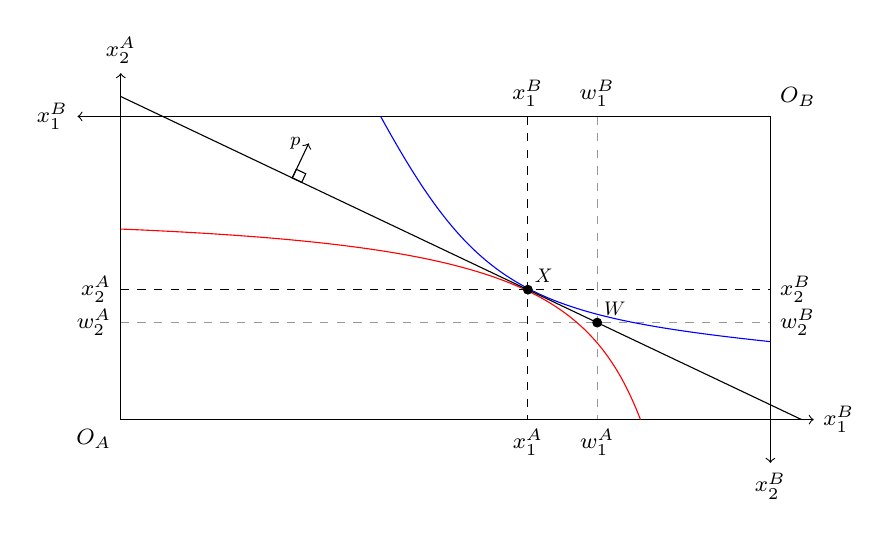
\begin{tikzpicture}[scale=1.1]
	% Formación de la caja
		% Consumidor A
			\draw[->] (0.5,0.5) node[align=center, below left] {\footnotesize $O_A$} -- (0.5,4.5) node[align=center, above] {\footnotesize $x_{2}^{A}$};
			\draw[->] (0.5,0.5) -- (8.5,0.5) node[align=center, right] {\footnotesize $x_{1}^{B}$};
		
		%Consumidor B
			\draw[->] (8,4) node[align=center, above right] {\footnotesize $O_B$} -- (0,4) node[align=center, left] {\footnotesize $x_{1}^{B}$};
			\draw[->] (8,4) -- (8,0) node[align=center, below] {\footnotesize $x_{2}^{B}$};
		
	% Intersección de una dotación
		% Demanda: X
			\draw[dashed] (5.2,4) node[above] {\footnotesize $x_{1}^{B}$} -- (5.2,0.5) node[below]{\footnotesize $x_{1}^{A}$};
			\draw[dashed] (0.5,2) node[left] {\footnotesize $x_{2}^{A}$} -- (8,2)node[right]{\footnotesize $x_{2}^{B}$};
		
		% Oferta: w
			\draw[dashed, opacity=0.4] (6,4) -- (6,0.5);
			\draw[dashed, opacity=0.4] (0.5,1.62)  -- (8,1.62);
			
				\draw (8,1.62)  node [right] {\footnotesize $w_{2}^{B}$};
				\draw (6,4)  node [above] {\footnotesize $w_{1}^{B}$};
				
				\draw (0.5,1.62)  node [left] {\footnotesize $w_{2}^{A}$};
				\draw (6,0.5)  node [below] {\footnotesize $w_{1}^{A}$};
	
	% Curvas de indiferencia
		\draw [blue] (3.5,4) .. controls (4.6,2) and (5.2,1.7) .. (8,1.4);
		\draw [red] (0.5,2.7) .. controls (4.915,2.515) and (5.915,2.015) .. (6.5,0.5);
	
	% Recta presupuestaria
		\draw (0.5,4.23) -- (8.36,0.5);
	
	% Puntos
		\draw[black, fill=black] (5.2,2) circle[radius=0.05] node [above right, scale=0.25mm] {$X$};
		\draw[black, fill=black] (6,1.62) circle[radius=0.05] node [above right, scale=0.25mm] {$W$};
		
	% Flecha y rectángulo
		\draw [->] (2.48,3.29) -- (2.67,3.69) node [left, scale = 0.3mm] {\footnotesize $p$};
		\draw [rotate around={-25:(2.48,3.29)}] (2.48,3.29) rectangle (2.6, 3.4);
\end{tikzpicture}
\end{frame}
%------------------------------------------------
\begin{frame}{Equilibrio General Walrasiano}
	Cada agente (considerando los precios como dados) se encuentra feliz con el resultado del intercambio (porque a esos precios y con su dotación inicial, cada agente no puede estar mejor), y además el intercambio puede realizarse (nadie está tratando de comprar o vender sin poder hacerlo)
\end{frame}
%------------------------------------------------
\begin{frame}{Equilibrio General Walrasiano}
	Como coinciden la pendientes de la recta presupuestal con las RMS, se tiene
		$$RMS_{x_1,x_2}^{A}\left( x_{1}^{A},x_{2}^{A}\right)  =  RMS_{x_1,x_2}^{B}\left( x_{1}^{B},x_{2}^{B}\right)  =  \frac{p_{1}}{p_{2}}$$
	Esto representa la condición de consumo eficiente (respuesta al problema de cómo asignar eficientemente los bienes entre los consumidores).
\end{frame}
%------------------------------------------------
\begin{frame}{Ley de Walras}
	Se define la función de exceso de demanda del bien $k$ para el consumidor $i$ como
		$$e_{ik}(p)=x_{ik}(p)-\overline{w}_{ik}$$
	Entonces
		$$e_{11}(p) + e_{21}(p)=0$$
		$$e_{12}(p) + e_{22}(p)=0$$
	Finalmente definimos la función de exceso de demanda agregada del bien $k$:
		$$z_{k}(p) = e_{1k}(p)+e_{2k}(p)$$
\end{frame}
%------------------------------------------------
\begin{frame}{Ley de Walras}
	El equilibrio walrasiano se puede definir entonces como un vector de precios $p^*$ y una asignación $x^*$, tal que
		$$z_{k}(p^*)=0, k=1,2$$
	Entonces, la Ley de Walras dice que la suma del valor de las funciones de exceso de demanda agregada es idénticamente igual a cero:
		$$\forall p, p_1z_1(p)+p_2z_2(p)=0$$
\end{frame}
%------------------------------------------------
\begin{frame}{Ley de Walras: Demostración}
		$$\forall p, p_1x_{11}(p)+p_2z_{12}(p)=p_1w_{11}+p_2w_{12}$$
	Para el consumidor 1, cualquier canasta de consumo, dado un sistema de precios, debe ser factible.\\
	Es decir: 
		$$p_1e_{11}(p)+p_2e_{12}(p)=0$$
	Lo mismo para el consumidor 2:
		$$p_1e_{21}(p)+p_2e_{22}(p)=0$$
	Sumando, obtenemos:
		$$p_1z_1(p)+p_2z_2(p)=0$$
\end{frame}
%------------------------------------------------
\begin{frame}{Ley de Walras: Implicancias}
	Una implicancia para una economía de intercambio de dos bienes es que si un mercado está en equilibrio, entonces el otro mercado también debe estar en equilibrio.
		\begin{itemize}
			\item ¿Qué sucede si, para precios positivos p1 y p2, hay un exceso de la cantidad ofertada del bien 1?
				$$x_{1}^{*A}+x_{1}^{*B}-w_{1}^{A}-w_{1}^{B} < 0$$
			\item Entonces:
				$$p_1\left(x_{1}^{*A}+x_{1}^{*B}-w_{1}^{A}-w_{1}^{B} \right) + p_2\left(x_{2}^{*A}+x_{2}^{*B}-w_{2}^{A}-w_{2}^{B} \right)=0$$
			\item Lo que implica que
				$$x_{2}^{*A}+x_{2}^{*B}-w_{2}^{A}-w_{2}^{B} > 0$$
		\end{itemize}
	Una segunda implicancia de la Ley de Walras para una economía de intercamio de dos bienes es que un exceso de oferta en un mercado implica exceso de demanda en el otro mercado.
\end{frame}